%%%%%%%%%%%%%%%%%%%%%%%%%%%%%%%%%%%%%%%%%%%%%%%%%%%%%%%%%%%%%%%%%%%%%
% LaTeX Template: 
% 
%%%%%%%%%%%%%%%%%%%%%%%%%%%%%%%%%%%%%%%%%%%%%%%%%%%%%%%%%%%%%%%%%%%%%%

\documentclass[12pt]{report}

% Layout and spacing
\usepackage[myheadings]{fullpage}
\usepackage{fancyhdr}
\usepackage{graphicx, wrapfig, setspace, booktabs, multirow}
\usepackage[font=small, labelfont=bf]{caption}
\usepackage{fourier}
\usepackage{microtype}
\usepackage[english]{babel}
\usepackage{sectsty}
\usepackage{url}
\usepackage{alltt}
\usepackage{amsmath}
\usepackage{color}
\usepackage{csquotes}  % Required for APA with biblatex

% Bibliography: APA 7th with clickable links, no backref page links
\usepackage[
  style=apa,
  backend=biber,
  doi=true,
  url=true,
  hyperref=true,
  backref=false,
  backrefstyle=none
]{biblatex}
\DeclareLanguageMapping{english}{english-apa}
\addbibresource{references.bib}

% Prevent page numbers in bibliography from becoming hyperlinks
\DeclareFieldFormat{pagetotal}{#1}
\DeclareFieldFormat{pages}{#1}
\DeclareFieldFormat{eprint:pages}{#1}
\DeclareFieldFormat{eprint:pagetotal}{#1}
% Force DOI links to display as full URLs
\DeclareFieldFormat{doi}{\url{https://doi.org/#1}}

% Fonts and encoding
\usepackage[T1]{fontenc}

% Final formatting
\usepackage{lastpage}
\usepackage{subfigure}
\onehalfspacing
\setcounter{tocdepth}{5}
\setcounter{secnumdepth}{5}
\renewcommand\thesection{\arabic{section}}

% Custom command
\newcommand{\HRule}[1]{\rule{\linewidth}{#1}}


%-------------------------------------------------------------------------------
% HEADER & FOOTER
%-------------------------------------------------------------------------------
\pagestyle{fancy}
\fancyhf{}
\setlength\headheight{15pt}
\fancyhead[L]{CSCI 499 Senior Project II}
\fancyhead[R]{Final Report}
\fancyfoot[R]{Page \thepage\ of \pageref{LastPage}}
%-------------------------------------------------------------------------------
% TITLE PAGE
%-------------------------------------------------------------------------------

\begin{document}


\title{ \normalsize \textsc{Senior Project II (SPRING 2025)\\Final Report}
		\HRule{0.5pt} \\
		\LARGE \textbf{\uppercase{Retrieval Augmented Generation for Resume Analysis}}
		\HRule{2pt} \\ [0.5cm]
		\normalsize \vspace*{5\baselineskip}}
		
\date{}

\author{Hugh Smith (N00296454, hubert.smith@udc.edu)\\
		Department of Computer Science and Information Technology\\
		University of the District of Columbia\\
		4200 Connecticut Avenue NW\\
		Washington, DC 20008}
\maketitle

\tableofcontents

\thispagestyle{empty} %% removing page number

\newpage

%-------------------------------------------------------------------------------
% Section title formatting
\sectionfont{\scshape}
%-------------------------------------------------------------------------------

%-------------------------------------------------------------------------------
% BODY
%-------------------------------------------------------------------------------

%-------------------------------------------------------------------------------
\section{Project Summary}

The job market has become rough for applicants and companies looking to hire. Recruiters must sift through hundreds, if not thousands, of resumes to find a good match for a role, often relying on outdated keyword-based systems that do not capture the deeper nuances of candidate profiles. To address this challenge, we have designed an innovative application that leverages advanced Artificial Intelligence (AI) techniques, specifically Retrieval-Augmented Generation (RAG), to transform how resumes are searched, analyzed, and matched.

%-------------------------------------------------------------------------------
\section{Introduction}

This project addresses modern recruitment's increasing complexity, where job seekers and hiring companies face significant challenges. The recruitment process often involves sifting through numerous resumes, creating a significant bottleneck for hiring managers attempting to efficiently identify suitable candidates. This problem is further exacerbated by the limitations of traditional keyword-based search systems, which struggle to capture the nuances of natural language and frequently overlook qualified applicants whose resumes may not contain specific keywords despite possessing relevant skills and experience. These inefficiencies in the hiring process lead to missed opportunities for both candidates and employers, preventing organizational growth and individual career progression. Crucially, handling sensitive personal data within resumes raises significant privacy concerns that this project directly addresses. This project aims to design and implement a Retrieval Aggregated Generation (RAG) system to revolutionize resume analysis and matching while prioritizing candidate privacy. This system will leverage advanced AI techniques to go beyond simple keyword matching, enabling a more nuanced understanding of candidate experience and qualifications through natural language understanding and contextual analysis. A key focus of this project is to implement a privacy-preserving information retrieval mechanism. Using advanced techniques, our aim is to perform semantic searches and matching without directly exposing sensitive personal information contained within resumes. This approach allows for efficient and accurate matching while minimizing the risk of data breaches and ensuring compliance with privacy regulations. 
This project will explore the application of RAG architecture, coupled with this privacy-preserving retrieval method, to effectively retrieve relevant information from a corpus of resumes and generate insightful comparisons against given job descriptions. This project will focus on the design, implementation, and evaluation of this RAG-based solution, aiming to demonstrate its potential to significantly improve the efficiency and effectiveness of the resume screening process within HR departments, ultimately leading to better hiring outcomes for both employers and job seekers while upholding stringent privacy standards. 
%-------------------------------------------------------------------------------

\begin{tabular}{ |p{4cm}||p{3cm}|p{3cm}|p{3cm}| }
  \hline
  \multicolumn{4}{|c|}{Project Timeline} \\
  \hline
  \textbf{Task} & \textbf{Start} & \textbf{End} & \textbf{Duration} \\
  \hline
  \multicolumn{4}{|c|}{Phase 1: Research and Exploration} \\
  \hline
  RAG Research & Sep 2 & Sep 9 & 1 Week \\
  \hline
  Model Exploration & Sep 9 & Sep 16 & 1 Week \\
  \hline
  Code Analysis & Sep 16 & Sep 27 & $\sim$1.5 Weeks \\
  \hline
  SLM Research & Sep 30 & Oct 4 & $\sim$1 Week \\
  \hline
  PHI-3 Testing & Oct 7 & Oct 11 & $\sim$1 Week \\
  \hline
  PDF Test Case & Oct 14 & Oct 18 & $\sim$1 Week \\
  \hline
  AI Expert Consultation & Oct 29 & Oct 29 & 1 Day \\
  \hline
  \multicolumn{4}{|c|}{Phase 2: Implementation and Design} \\
  \hline
  Dataset Acquisition & Oct 30 & Nov 1 & $\sim$1 Week \\
  \hline
  RAG Architecture & Nov 1 & Nov 5 & $\sim$1 Week \\
  \hline
  GUI Exploration & Jan 15 & Jan 19 & 1 Week \\
  \hline
  Code Adaptation & Feb 1 & Feb 14 & 2 Weeks \\
  \hline
  Code Refactoring & Feb 17 & Feb 29 & 2 Weeks \\
  \hline
  Chatbot Development & Mar 1 & Mar 21 & 3 Weeks \\
  \hline
  Authentication Setup & Mar 22 & Apr 5 & 2 Weeks \\
  \hline
  \multicolumn{4}{|c|}{Phase 3: Finalization and Testing} \\
  \hline
  End-to-End Testing & Apr 8 & Apr 15 & 1 Week \\
  \hline
  MVP Development & Apr 16 & Apr 26 & $\sim$1.5 Weeks \\
  \hline
 \end{tabular}

%-------------------------------------------------------------------------------
\section{Previous work}

The challenge of efficiently and effectively matching resumes to job descriptions has been a subject of ongoing research and development within the Natural Language Processing (NLP) and Information Retrieval (IR) fields. \parencite{rojas-galeano-2022} Traditional approaches have often relied on keyword-based matching, which, as discussed earlier, needs to be improved in capturing the semantic nuances of both resumes and job descriptions. These systems often fail to recognize synonyms, related skills, or the context in which keywords appear, leading to false positives and false negatives in candidate selection.\parencite{gawande-2024}

Recent efforts have explored more sophisticated NLP techniques, including Semantic Analysis, Named Entity Recognition, and Topic Modeling. These methods aim to extract deeper meaning from textual data, allowing for more accurate matching based on skills, experience, and qualifications. For example, Word2Vec and GloVe have been employed to create word embeddings, representing words as vectors in a high-dimensional space where semantically similar words are located closer together. This allows systems to identify matches even when different wording is used. \parencite{alderham-2024}

The advent of transformer-based models, such as Bidirectional Encoder Representations from Transformers (BERT) and its variants, has further advanced the field. These models excel at understanding context and capturing complex relationships within text, significantly improving various NLP tasks, including text classification, question answering, and semantic similarity. Applying these models to resume matching allows for a more comprehensive understanding of candidate profiles.

However, privacy concerns have become paramount with the increasing use of sensitive personal information in resume analysis. Traditional methods of storing and processing resume data often involve storing the raw text, which raises risks of data breaches and misuse. This is where the concept of privacy-preserving information retrieval becomes crucial. Recent research has explored using vector databases and embedding models to address these privacy concerns. \parencite{he-2025} By converting textual data into vector embeddings and storing only these embeddings in the database, the system can perform semantic searches without directly accessing or storing the raw, sensitive data. This approach significantly improves data protection and aligns with growing privacy regulations. \parencite{boppana-no-date} Techniques like federated learning and differential privacy have also been explored with vector databases to enhance privacy by allowing models to learn from decentralized data without directly sharing sensitive information. This project builds upon these advancements by explicitly focusing on applying a RAG architecture combined with a privacy-preserving vector database approach, leveraging the benefits of contextual understanding while mitigating privacy risks. Using a vector database like Pinecone, represents a specific implementation of this privacy-preserving strategy, allowing for efficient similarity searches without compromising sensitive data, a topic we will explore further in subsequent sections.


%-------------------------------------------------------------------------------
\section{Project Approach}

This project systematically designs and implements a privacy-preserving RAG system for resume analysis. The core methodology can be broken down into the following key components:
\begin{enumerate}

    \item Understanding and Implementing RAG: The foundation of this project lies in a thorough understanding of the Retrieval-Augmented Generation paradigm. RAG combines the strengths of information retrieval and generative language models. The retrieval component is responsible for fetching relevant context from a knowledge base (in this case, a collection of resumes), while the generation component uses this retrieved-context to generate a response or perform a specific task, such as comparing a resume against a preprogrammed job description. This project will explore different retrieval strategies and generation techniques to optimize the system's performance.
    \item Dataset Acquisition and Preparation: A crucial step in any machine learning project is the acquisition and preparation of a suitable dataset. For this project, a comprehensive dataset of over 3000 PDF resumes sourced from Kaggle was selected. This dataset encompasses various career fields and resume formats, providing a realistic and challenging testbed for the RAG system. The PDF format presents an additional challenge, requiring robust PDF parsing and text extraction techniques to convert the resume content into a usable format for the model. This preprocessing step is essential for ensuring the quality and consistency of the data used for retrieval and generation.
    \item User Interface Development: To ensure the RAG system is accessible and intuitive, a web-based interface was considered essential. Initially, frameworks such as Gradio and Streamlit were explored due to their low-code interfaces and rapid prototyping capabilities. While Streamlit was briefly used in the early stages for proof-of-concept development, we ultimately transitioned to a custom-built solution using TypeScript, React, and Shadcn UI. This shift provided greater flexibility, scalability, and design control—allowing for more advanced user interactions, seamless integration with authentication (Clerk), and an overall production-ready architecture.
    \item Security and Authentication: Given the sensitive nature of the data involved, implementing robust security measures is paramount. The system employs Clerk for user authentication, ensuring that only authorized users can access the application and its features. This authentication layer is critical for protecting sensitive personal information contained within resumes and maintaining compliance with privacy regulations. The integration of Clerk provides a secure and user-friendly authentication experience, allowing users to log in seamlessly while ensuring their data remains protected.
    \item Privacy and Ethical Considerations: As mentioned above, a central focus of this project is addressing the privacy implications of handling sensitive personal information contained within resumes. Traditional methods of storing and processing resume data raise significant privacy concerns. This project aims to mitigate these risks by employing additional privacy-preserving techniques, primarily through vector embeddings and a specialized vector database. The system can perform semantic searches and comparisons without directly accessing or storing the raw, sensitive data by converting resume text into vector representations. This approach minimizes the risk of data breaches and aligns with growing privacy regulations. Furthermore, ethical considerations surrounding bias in AI models and fairness in hiring practices will be carefully considered throughout the project lifecycle. This includes evaluating the model's performance across different demographic groups and implementing strategies to mitigate potential biases.

\end{enumerate}
    This multi-faceted approach, encompassing RAG implementation, comprehensive dataset utilization, user-friendly interface development, and a strong emphasis on privacy and ethical considerations, forms the core of this project. 

\subsection{Retrieval-Augmented Generation Overview}
Retrieval-augmented generation (RAG) offers a compelling approach to the complex resume analysis and matching task. Combining the strengths of information retrieval and generative language models, RAG addresses the limitations of traditional keyword-based systems and provides a more nuanced and context-aware understanding of candidate profiles. This section outlines the RAG paradigm and its specific application within this project, focusing on how it enhances resume analysis.
The core idea behind RAG is to enhance the generation process with relevant information retrieved from an external knowledge source. In the context of resume analysis, this knowledge source is a collection of resumes and job descriptions. The RAG process can be broken down as follows:

\begin{enumerate}
    \item \textbf{Ouery/input:} The process begins with a user query or input. For this project the input is a resumes that needs to be analyzed against a job description. The input can be in the form of a natural language question or a specific task, such as comparing a resume to a job description.
    \item \textbf{Retrieval:} A retrieval component searches a large corpus of documents (our knowledge base) for information relevant to the input query. This project’s knowledge base consists of a dataset of over 3000 PDF resumes sourced from Kaggle. The retrieval process aims to identify resumes (or relevant sections within resumes) that contain skills, experience, keywords, or other information pertinent to the job description (or the provided resume). For example, if the job description requires "project management experience," the retrieval component will search for resumes that explicitly mention "project management" or related terms like "project leadership," "team coordination," or specific project management methodologies.
    \item \textbf{Augmentation:} The retrieved information is then combined with the original input query. This augmented input provides the generative model with the necessary context to perform the analysis. For example, if a job description requires proficiency in Python and the retrieval step finds several resumes mentioning Python experience, this information is combined with the job description and passed to the generative model.
    \item \textbf{Generation:} Once the relevant context is retrieved, the generative language model uses this information to generate responses or perform specific tasks. In this project, the generation component will be responsible for comparing resumes against job descriptions, providing insights into how well a candidate's qualifications align with the requirements of a given role.
    \item \textbf{Integration:} The integration of retrieval and generation is a key aspect of RAG. By combining these two components, the system can leverage the strengths of both approaches. The retrieval component ensures that the generative model has access to relevant and up-to-date information, while the generation component provides a flexible and context-aware response. 
    \item \textbf{Privacy Preservation:} A critical consideration in this project is the privacy of sensitive personal information contained within resumes. The RAG system will employ privacy-preserving techniques, such as vector embeddings and a specialized vector database, to ensure that sensitive data is not directly accessed or stored. This approach minimizes the risk of data breaches and aligns with growing privacy regulations.
\end{enumerate}

The RAG architecture allows for a more sophisticated and context-aware analysis of resumes, enabling the system to understand the nuances of candidate profiles and job requirements. By leveraging the strengths of both retrieval and generation, RAG can provide more accurate and relevant insights into candidate qualifications, ultimately improving the efficiency and effectiveness of the resume screening process.

\subsection{RAG Architecture}
The diagram below illustrates the RAG architecture and its components:
\begin{figure}[h]
    \centering
    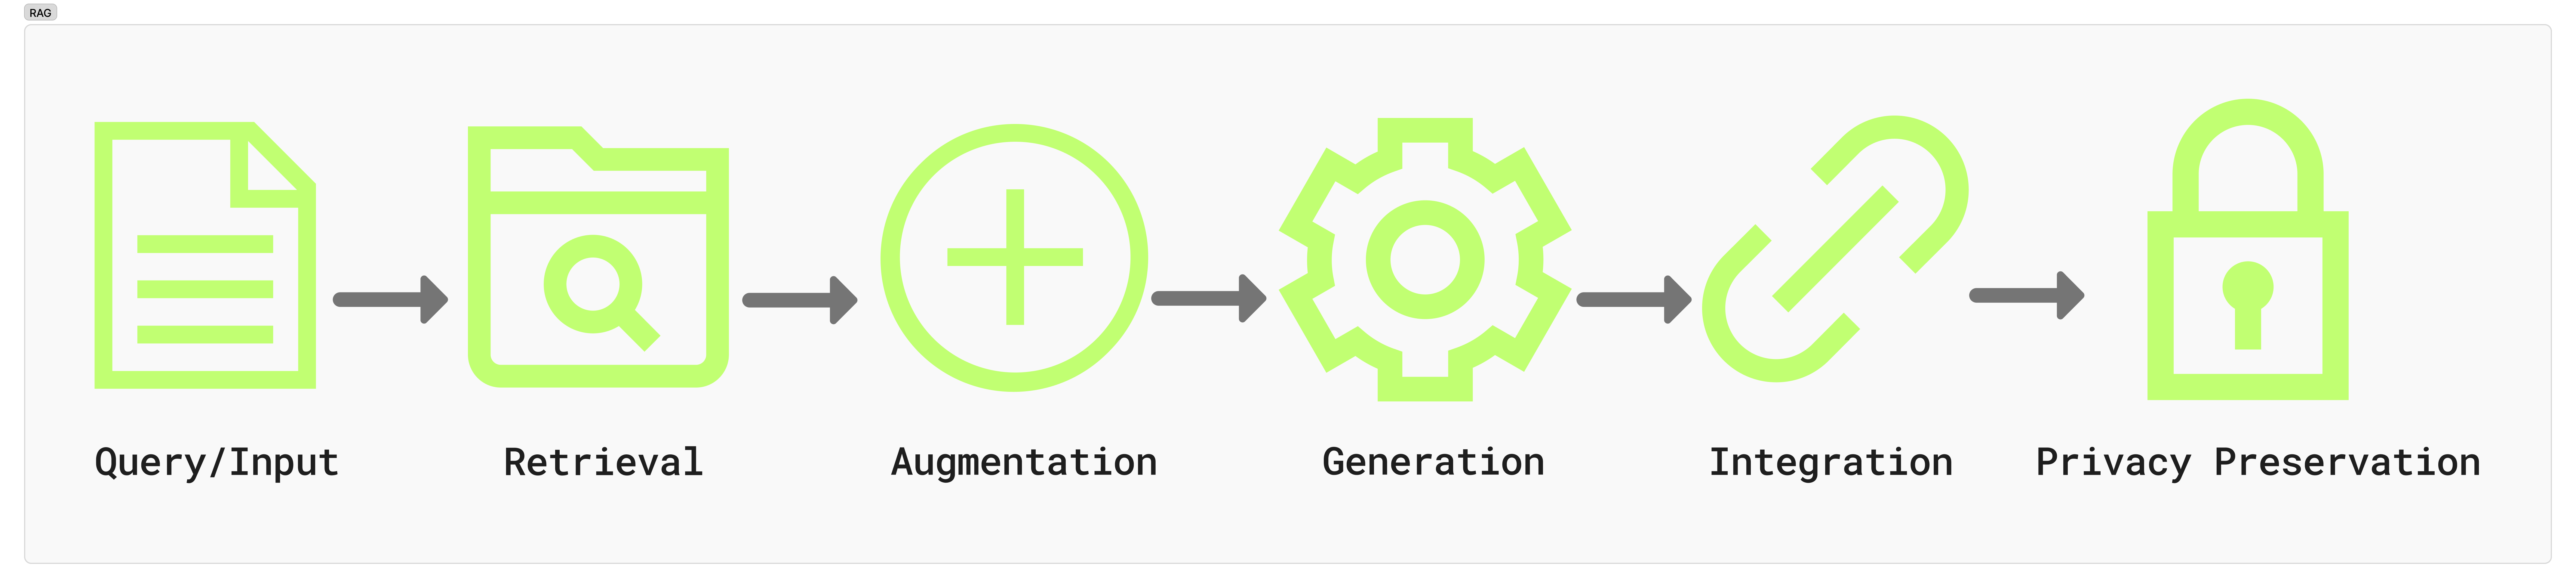
\includegraphics[width=1\textwidth]{images/RAG_Diagrams.png}
    \caption{Shows the basic idea behind Retrieval Augmented Generation (RAG) and how it works.}
    \label{fig:rag_diagram}
\end{figure}

By incorporating a retrieval step, RAG offers several key advantage for this project: 
\begin{enumerate}
    \item \textbf{Improved Accuracy and Relecance:} By grounding the analysis in a wide array of resumes, RAG can provide more accurate and relevant insights into candidate qualifications. This is particularly important in the context of resume analysis, where the nuances of language and context play a significant role in understanding a candidate's experience and skills.
    \item \textbf{Dynamic Knowledge Base:} The retrieval component enables the system to access a dynamic knowledge base of resumes, ensuring that the analysis is based on up-to-date information.
    \item \textbf{Privacy Preservation:} By employing privacy-preserving techniques, RAG can perform semantic searches and comparisons without directly accessing or storing sensitive personal information.
    \item \textbf{Flexibility and Adaptability:} The RAG architecture allows for flexibility in adapting to different tasks and domains, making it suitable for various recruitment scenarios.
\end{enumerate}

RAG provides a powerful and adaptable framework for this resume analysis and matching project, offering a significant improvement over traditional methods by leveraging the power of both retrieval and generation.

\section{Dataset Acquisition and Preparation}

The effectiveness of a Retrieval Augmented Generation (RAG) system relies heavily on the quality and comprehensiveness of its knowledge base. In this project, the dataset of over 3000 resumes serves as this crucial knowledgebase, providing the foundation for robust and accurate resume analysis.

The dataset's dual format, encompassing both string and PDF representations of resumes, is particularly beneficial. The string format allows for efficient indexing and retrieval of textual information, which is vital for the RAG pipeline. The inclusion of PDFs reflects real-world scenarios and necessitates implementing robust PDF parsing techniques, ensuring the system can handle the diverse formats encountered in recruitment workflows.

The dataset was sourced from Kaggle, a well-known platform for data science and machine learning resources. Crucially, the dataset exhibits significant diversity across 24 distinct job categories. This breadth of categories, from common fields like Information Technology, Engineering, and Healthcare to more specialized areas such as Digital Media, Fitness, and Public Relations, is essential for the project's goals. In a RAG system, the retrieval component searches this knowledge base to find relevant context for the generation component. The diversity of the dataset ensures that the system can effectively retrieve relevant information for a wide range of job descriptions and candidate profiles.
For instance, if a user provides a job description for a "Software Engineer," the RAG system will search the resume database, retrieving resumes categorized as "Information-Technology" or "Engineering," as well as resumes containing relevant keywords like "programming," "software development," or specific programming languages. This retrieved information then augments the input to the generation component, allowing it to make informed comparisons and assessments.

Therefore, the dataset's diversity is not primarily about training a statistical model to generalize from examples, as in traditional machine learning. Instead, it's about providing a rich and representative collection of resumes that the RAG system can effectively search and utilize to provide contextually relevant and accurate analysis for various job descriptions and candidate profiles. This robust and diverse knowledge base empowers the RAG system to perform effective resume analysis and matching.

\section{User Interface Development}
The user interface (UI) of the RAG system is a critical component that directly impacts user experience and interaction with the application. Initially, low-code frameworks like Gradio and Streamlit were considered for rapid prototyping. However, these frameworks were ultimately deemed insufficient for the project's long-term goals, particularly regarding customization and scalability.

A crucial aspect of this project is providing a user-friendly and intuitive interface that allows the user to interact seamlessly with the RAG system. Early in the project, Gradio and Streamlit were considered potential frameworks for building this interface. This section provides an overview of each framework, weighing their respective pros and cons in the context of this specific project, ultimately explaining the pivot towards Streamlit.
\subsection{Gradio vs. Streamlit}
Gradio is a Python library specifically designed for quickly creating interactive interfaces for machine learning models. It excels at creating simple demos and sharing models with others.
\begin{itemize}
    \item \textbf{Pros:}
        \begin{itemize}
            \item \textbf{Ease of Use:} Gradio is incredibly easy to set up and use, especially for showcasing individual model functionalities. It requires minimal code to create basic interfaces.
            \item \textbf{Built-in Components:} Gradio provides a variety of built-in components for input and output, making it easy to create interactive demos without extensive customization.
            \item \textbf{Sharing capabilities:} Gradio allows for easy sharing of interfaces via links, making it convenient for collaboration and feedback.
        \end{itemize}
    \item \textbf{Cons:}
        \begin{itemize}
            \item Limited customization options for UI design and layout.
            \item Not suitable for complex applications requiring extensive interactivity.
        \end{itemize}
\end{itemize}
Streamlit is an open-source Python library that makes it easy to create and share beutiful web applications for machine learning and data science projects. It is designed for building data-driven applications quickly and efficiently.
\begin{itemize}
    \item \textbf{Pros:}
        \begin{itemize}
            \item \textbf{Flexibility and Customization:} Streamlit provides much greater control over the UI layout, styling, and interactivity. It allows for building more complex and customized applications.
            \item \textbf{Data Visualization:} Streamlit offers excellent support for data visualization, making it suitable for displaying results and insights from the RAG system.
            \item \textbf{Python Development:} Streamlit uses a Pythonic approach, making it easy for data scientists and developers familiar with Python to build web apps.
            \item \textbf{Caching Mechanism:} Streamlit includes built-in caching, which can significantly improve performance, especially for computationally intensive tasks.
            
        \end{itemize}
    \item \textbf{Cons:}
        \begin{itemize}
            \item Steeper learning curve compared to Gradio, especially for users unfamiliar with web development concepts.
            \item More setup time required to create a fully functional application.
        \end{itemize}
\end{itemize}
\subsection{Final Decision}
Ultimately, the decision was made to not work with either Gradio or Streamlit. The project pivoted towards a custom-built solution using TypeScript, React, and Shadcn UI. This decision was driven by the need for greater flexibility, scalability, and design control. The custom-built solution allows for more advanced user interactions, seamless integration with authentication (Clerk), and an overall production-ready architecture. In the early part of the project, Gradio was used briefly to provide a proof-of-concept for the RAG system. However, as the project evolved, it became clear that a more robust and customizable solution was needed to meet the project's long-term goals.

This approach offers several advantages:
\begin{itemize}
    \item \textbf{Customization:} A custom-built solution allows for complete control over the UI design and functionality, enabling the creation of a tailored user experience that meets the specific needs of the RAG system. This can be especially important if this were to go to market. Some organizations may have specific requirements for their user interfaces, and a custom solution allows for that.
    \item \textbf{Scalability:} The use of modern web technologies like TypeScript and React ensures that the application can scale effectively as user demand grows.
    \item \textbf{Integration:} The custom solution allows for seamless integration with backend services, ensuring a smooth user experience.
    \item \textbf{Production-Ready:} By building a production-ready architecture from the ground up, the project can ensure reliability, performance, and maintainability in the long term.
\end{itemize}

\section{Ethical Considerations}
Beyond privacy, this project also addresses broader ethical considerations related to the use of AI in recruitment:
\begin{itemize}
    \item \textbf{Bias Mitigation:} AI models can inadvertently perpetuate biases present in the data they are trained on. This project will carefully evaluate the model's performance across different demographic groups and implement strategies to mitigate potential biases.
    \item \textbf{Fairness and Transparency:} The project aims to promote fairness in hiring practices by providing a transparent and objective assessment of candidate suitability. With its retrieval component, the RAG approach offers a degree of explainability by providing the retrieved context as evidence for its generated outputs.
    \item \textbf{Human Oversight:} While automation can improve efficiency, human oversight remains crucial. The project emphasizes the importance of human review in the final hiring decision, ensuring that the AI system is used to assist, not replace, human judgment. 
\end{itemize}

\section{Architecture Overview}
This system is designed with a modular architecture that ensures security, scalability, and flexibility. As mentioned earlier, users will have to authenticate themselves using Clerk, a third-party authentication service. This integration is crucial for protecting sensitive personal information contained within resumes and maintaining compliance with privacy regulations. After authentication, user can  upload multiple or a single resume, and select from a preprogrammed job description. The system will then parse the resumes and job descriptions, extracting relevant information for analysis. The RAG architecture will be employed to retrieve relevant context from the knowledge base (the dataset of resumes) and generate insights based on this context. The retrieved information will be combined with the original input query to provide a comprehensive analysis of how well a candidate's qualifications align with the requirements of a given role. Here is a view of the current architecture:

\begin{figure}[h]
    \centering
    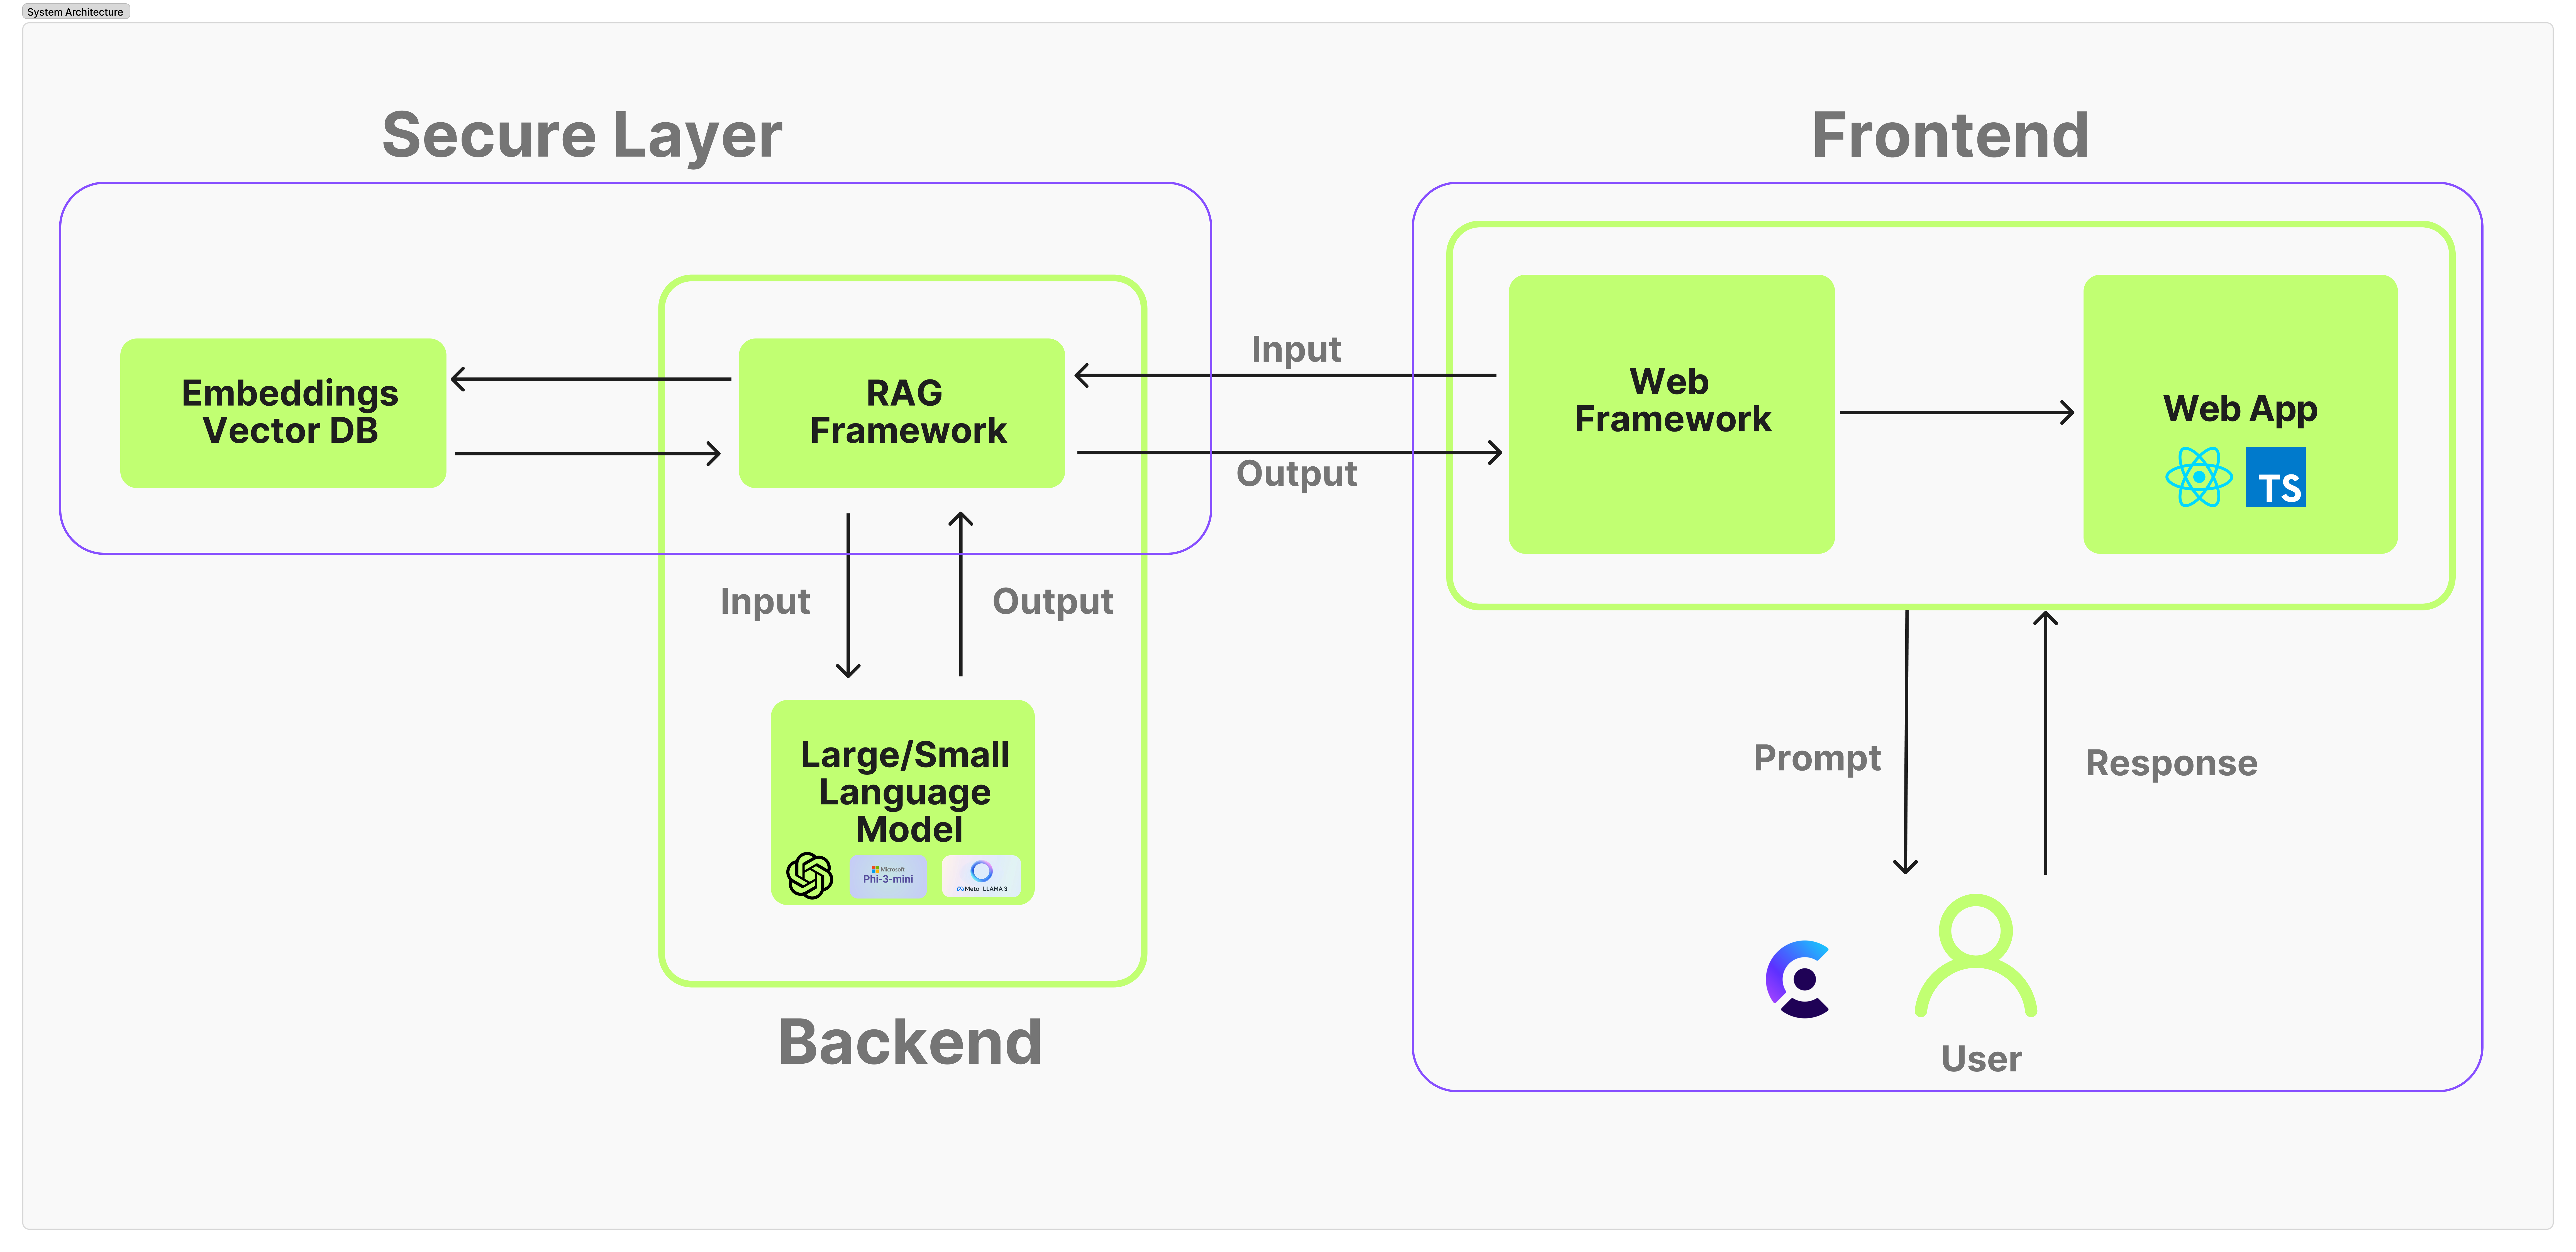
\includegraphics[width=1\textwidth]{images/System_Arch.png}
    \caption{Shows the architecture of the system.}
    \label{fig:architecture_diagram}
\end{figure}


\section{Conclusion}
This project aimed to create a Retrieval-Augmented Generation (RAG) system for more nuanced, ethical, and privacy-conscious resume analysis and matching. Moving beyond traditional keyword-based methods, the system leverages advanced language models and a large dataset of over 2,400 resumes to deliver context-aware candidate-to-job matching. A key innovation is the integration of RAG, which combines data retrieval with generative modeling. This approach enables a deeper understanding of candidate profiles and job descriptions, allowing the system to capture context and semantics rather than relying solely on keyword occurrences. Privacy was a central focus throughout development. Instead of working directly with raw, sensitive personal information, the system uses vector embeddings and a specialized vector database like Pinecone. This method reduces exposure to sensitive data and lowers the risk of breaches, ensuring compliance with privacy regulations and fostering user trust. Beyond privacy, the project also addressed ethical considerations such as bias, fairness, and transparency. It acknowledges the importance of human oversight to maintain integrity and promote equitable hiring practices. The final solution, presented through a Streamlit interface, offers a user-friendly experience for recruiters. Users can input job descriptions or resumes and quickly receive insightful, context-aware matching results. This seamless experience supports the practical integration of the system into real-world recruitment workflows. 



%-------------------------------------------------------------------------------
% REFERENCES
%-------------------------------------------------------------------------------

\printbibliography
\addcontentsline{toc}{section}{Bibliography}

\end{document}
